%%%%%%%%%%%%%%%%%%%%%%%%%%%%%%%%%%%%%%%%%%%%%%%%%%%%%%%%%%%%%%%%%%% 
%                                                                 %
%                            CHAPTER                              %
%                                                                 %
%%%%%%%%%%%%%%%%%%%%%%%%%%%%%%%%%%%%%%%%%%%%%%%%%%%%%%%%%%%%%%%%%%% 
\chapter{Implementation}
\label{chapter:implementation}
This chapter is split into three sections. In the first section, we go over the structure of the algorithm. In the second and third sections, we go into detail about the two sub-research questions: how to construct the schema and how to populate the schema. 


% At this time we only have a PoC implementation, as such many details haven't been worked out yet. For example, the section on creating the schema is limited, as we only handle CSV files which require little to no schema. 

For the implementation, we assume that the mapping rules never map to a superset of the knowledge graph. 

The implementation is written in Python. As we seek to extend Morph-KGC we make use of its internal functions and the libraries to work with those, like pandas. Querying the knowledge graph is done with the SPARQLWrapper library.

\section{General structure}
The algorithm consists of 4 main parts: setting up, creating the schema, retrieving the data, and applying the data to the schema. Creating the schema and retrieving the data are the two main parts of the implementation, and are covered in their sections. Setting up consists of setting up the \acrshort{sparql} endpoint if necessary and processing the mapping files. Applying the data to the schema consists of applying the data of each iteration to the schema, and creating the output file. A graphical representation of the algorithm can be found in figure \ref{fig:algorithm}. A more formal representation can be found in algorithm \ref{alg:inversion}. The functions used in the algorithm are described in the relevant sections.

\begin{figure}[h]
    \centering
    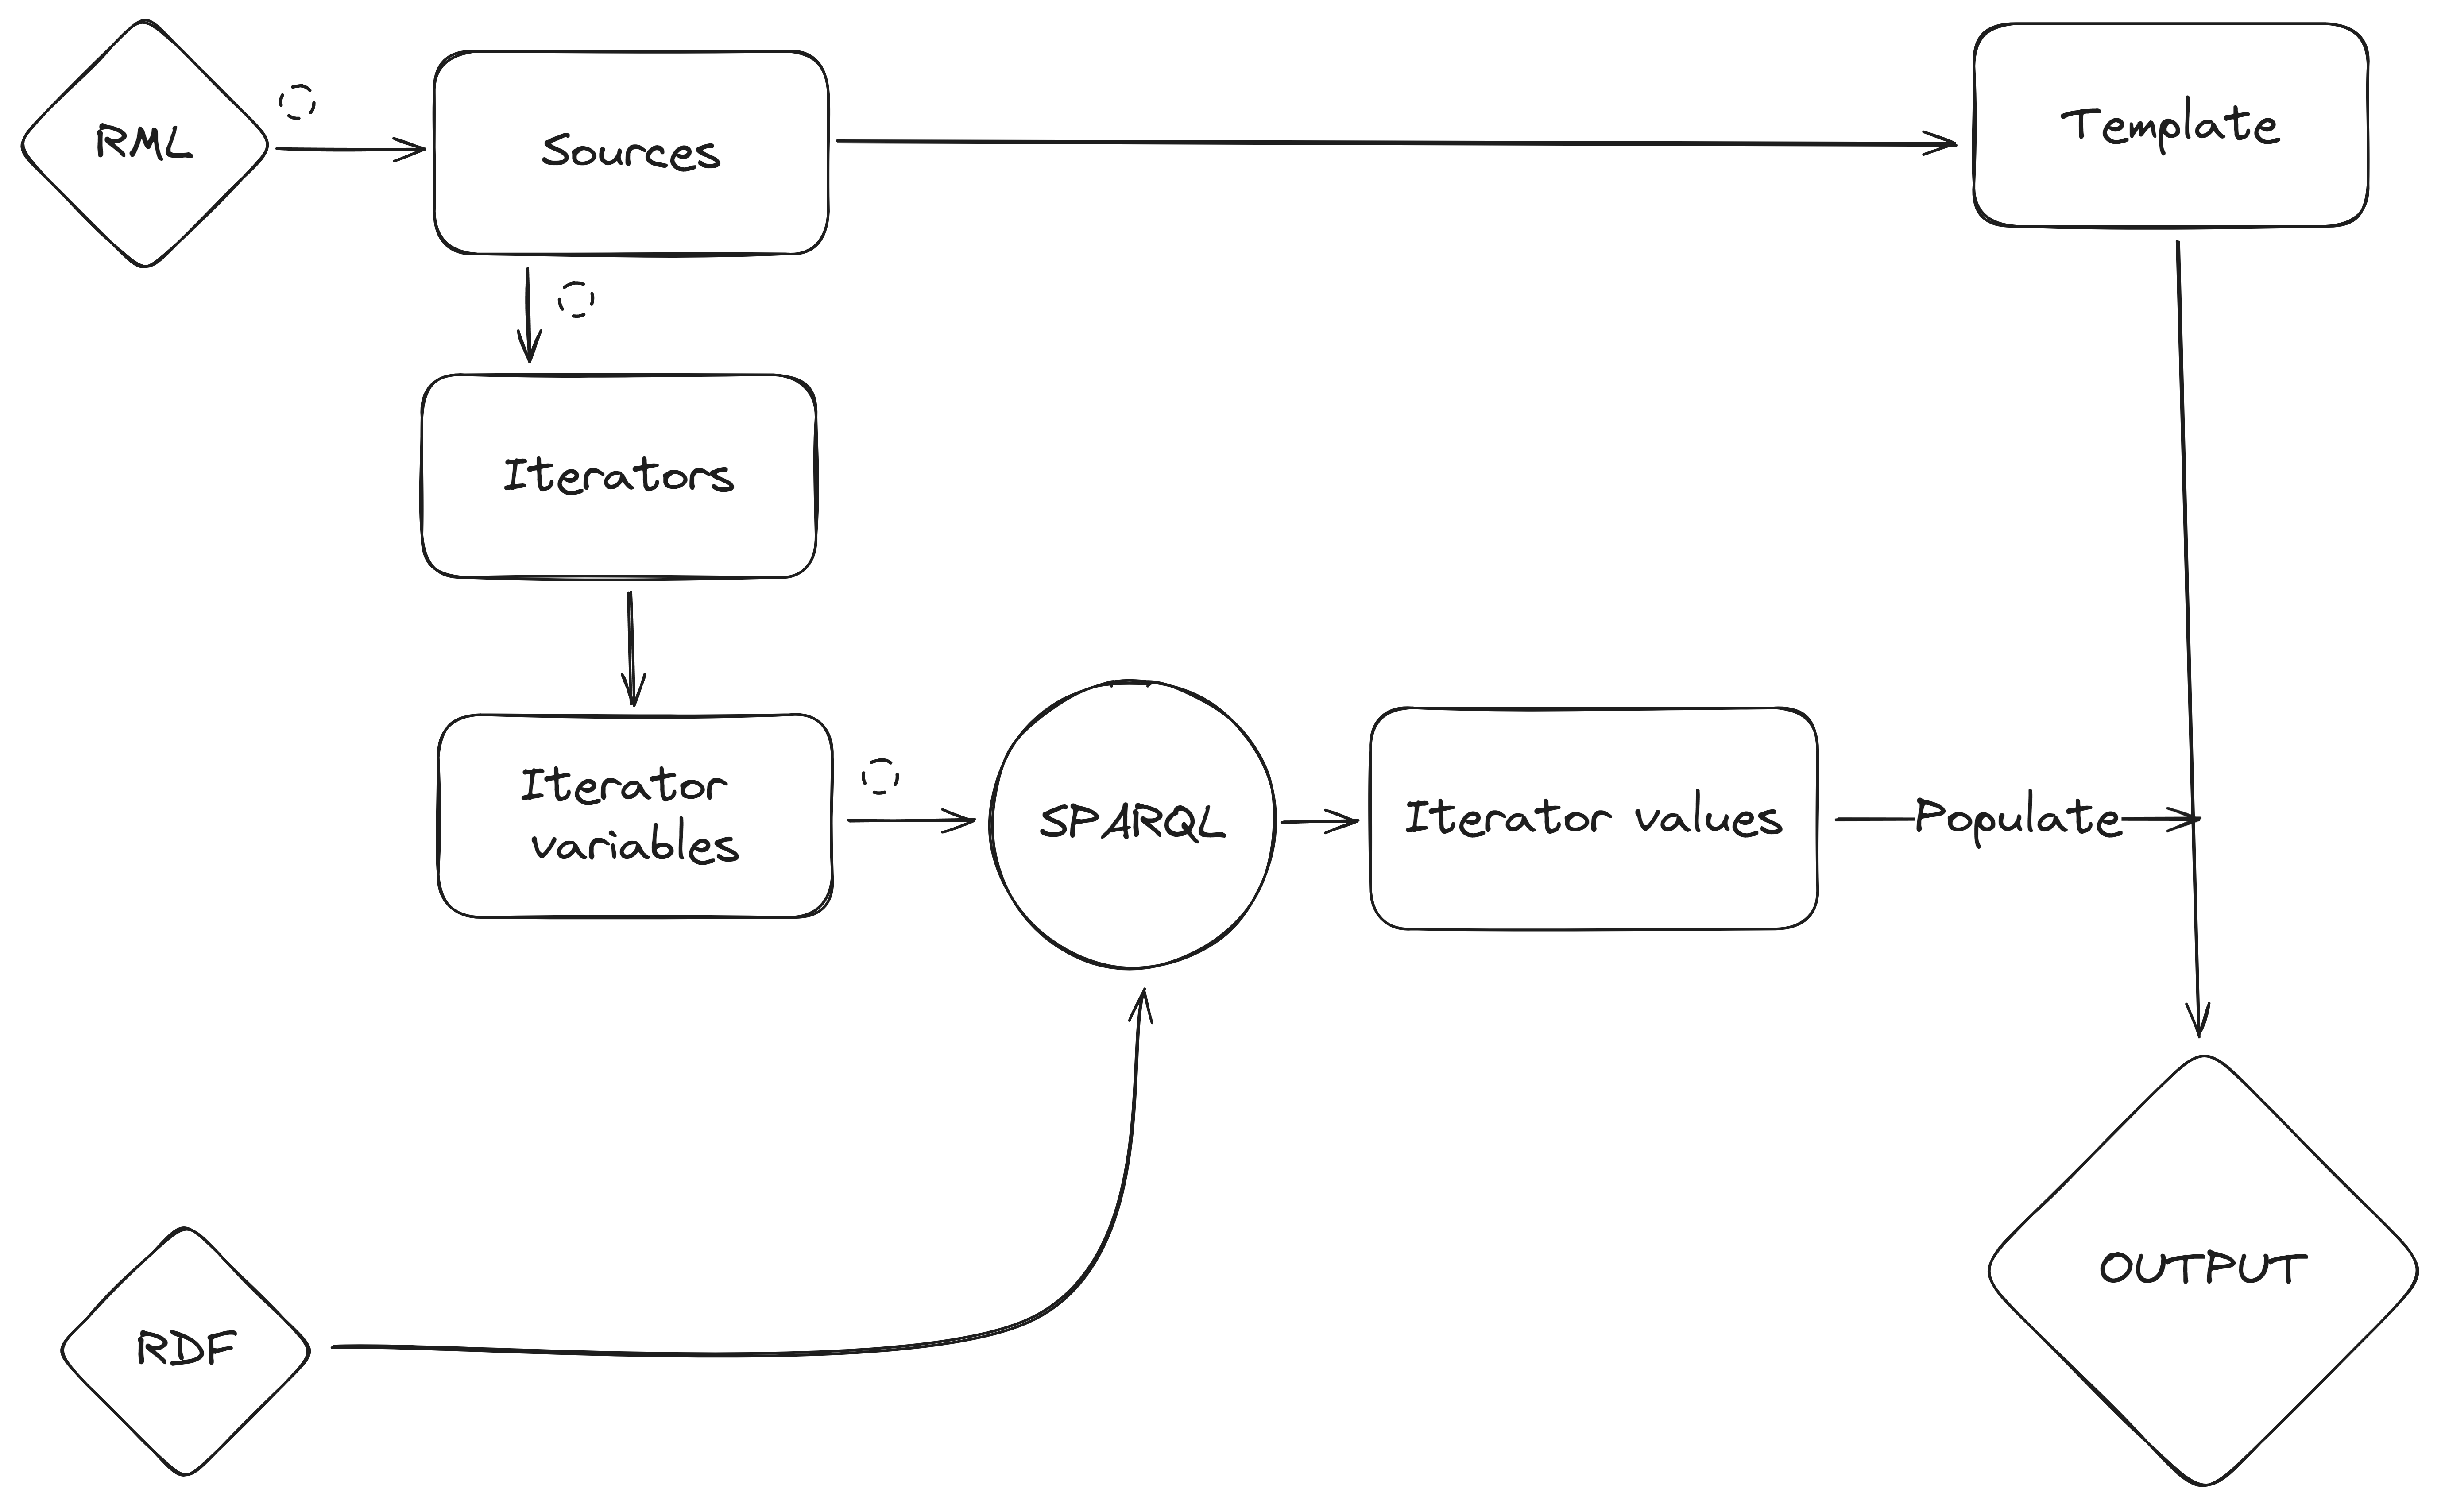
\includegraphics[width=\textwidth]{Chapter3/algorithm_flat.png}
    \caption{Simplified overview of the algorithm}
    \label{fig:algorithm}
\end{figure}

\begin{algorithm}
    \caption{Inversion algorithm}
    \label{alg:inversion}
    \begin{algorithmic}[1]
        \Require{$morph\_config$ is a morph-kgc config file describing the mapping files and output location}
        \State $config \gets load_config(morph\_config)$
        \State $mapping\_rules \gets retrieve\_mappings(config)$
        \State $mapping\_rules \gets add\_helper\_columns(mapping\_rules)$
        \State $graph\_location \gets config.get_output_file()$
        \State $graph\_endpoint \gets load\_graph(graph\_location)$
        \ForAll{$source, source\_rules \in mapping\_rules.groupby('source')$}
            \ForAll{$iterator, iterator\_rules \in source\_rules.groupby('iterator')$}
                \State $query \gets generate\_query(iterator\_rules)$
                \State $values[iterator] \gets graph.query(query)$
            \EndFor
            \State $templates \gets generate\_templates(source\_rules)$
            \State $source\_output \gets apply\_templates(templates, values)$
        \EndFor
    \end{algorithmic}
\end{algorithm}

% I made this as a joke, this is in no way readable so the algorithm is split over the sections
% \begin{algorithm}
%     \caption{Full inversion algorithm}
%     \label{alg:inversion}
%     \begin{algorithmic}[1]
%         \Require{$morph\_config$ is a morph-kgc config file describing the mapping files and output location}
%         \State $config \gets load_config(morph\_config)$
%         \State $mapping\_rules \gets retrieve\_mappings(config)$
%         \State $mapping\_rules \gets add\_helper\_columns(mapping\_rules)$
%         \State $graph\_location \gets config.get_output_file()$
%         \State $graph\_endpoint \gets load\_graph(graph\_location)$
%         \ForAll{$source, source\_rules \in mapping\_rules.groupby('source')$}
%             \ForAll{$iterator, iterator\_rules \in source\_rules.groupby('iterator')$}
%                 \ForAll{$subject, subject\_rules \in iterator\_rules.groupby('subject')$}
%                     \ForAll{$rule \in subject\_rules$}
%                         \If{$rule.is\_constant()$}
%                             \State $query\_lines.append(rule.to\_triple())$ 
%                         \ElsIf{$rule.is\_reference()$}
%                             \State $query\_lines.append(rule.to\_triple())$
%                         \ElsIf{$rule.is\_template()$}
%                             \State $query\_lines.append(test\_object\_regex(rule))$
%                             \State $remainder \gets rule['object\_map\_value']$
%                             \ForAll{$reference \in rule.get\_references()$}
%                                 \If{$remainder.empty()$}
%                                     \State $query\_lines.append(bind\_str\_after\_ref(reference)) $
%                                 \Else
%                                     \State $query\_lines.append(bind\_str\_after\_remainder()) $
%                                     \State $query\_lines.append(bind\_str\_before(reference)) $
%                                 \EndIf
%                                 \State $remainder \gets remainder - reference$
%                             \EndFor
%                         \EndIf
%                         \State $query \gets wrap\_query\_lines(query\_lines)$
%                     \EndFor                                
%                 \State $query \gets generate\_query(iterator\_rules)$
%                 \State $values[iterator] \gets graph\_endpoint.query(query)$
%                 \EndFor
%             \EndFor
%             \If{$source\_rules['source\_type'] == 'CSV'$}
%                 \State $source\_output \gets values[0]$
%             \EndIf
%         \EndFor
%     \end{algorithmic}
% \end{algorithm}

\subsection{Loading the mapping rules}
We start by loading the mapping rules from the mapping files. We use Morph-KGC's internal \texttt{retrieve\_mappings} function for this. This function takes a loaded config file (.ini format) as input, which specifies the location of the mapping files and various other settings for which we have little use as they are only used for the materialization process. When relevant later on we could add our settings to this config file.
The mappings are returned as a pandas DataFrame. As the pandas library has the functionality to group by columns, we can easily group the mapping rules by source and iterator later. An example of a single mapping rule (row in the DataFrame) can be found in listing \ref{lst:mapping_rule}.

\begin{lstlisting}[caption={Example of a mapping rule in Morph-KGC}, label={lst:mapping_rule}, captionpos=b, basicstyle=\small]
    source_name: DataSource1 
    triples_map_id: #TM0
    triples_map_type: http://w3id.org/rml/TriplesMap
    logical_source_type: http://w3id.org/rml/source
    logical_source_value: student.csv
    iterator: nan
    subject_map_type: http://w3id.org/rml/template
    subject_map_value: http://example.com/{Name}
    subject_termtype: http://w3id.org/rml/IRI
    predicate_map_type: http://w3id.org/rml/constant
    predicate_map_value: http://xmlns.com/foaf/0.1/name
    object_map_type: http://w3id.org/rml/reference
    object_map_value: Name
    object_termtype: http://w3id.org/rml/Literal
    object_datatype: nan
    object_language: nan
    graph_map_type: http://w3id.org/rml/constant
    graph_map_value: http://w3id.org/rml/defaultGraph
    subject_join_conditions: nan
    object_join_conditions: nan
    source_type: CSV
    mapping_partition: 1-1-1-1
\end{lstlisting}

\section{Contructing the schema}
\label{section:constructing_schema}
Constructing the schema is done by reversing the mapping rules' source. We do this using the iterator and the mapping rule's references. \acrshort{rml} supports many different types of sources and referenceFormulations. We will implement the CSV, xPath, and JSONPath referenceFormulations. Not every source is a file, so for query-based sources, we will generate the query output. In a later stage, we could look into taking it a step further, generating the actual source behind those intermediate results.

As each referenceFormulation has its reference syntax, we will have to tailor the implementation to each referenceFormulation. For the PoC, we only implement the CSV referenceFormulation. 

\subsection{CSV}
\label{subsection:csv}
The CSV referenceFormulation is the simplest of the three as it describes a simple two-dimensional table, with columns having the names of the references and rows being the iterated values. The example TriplesMap in listing \ref{lst:csv_file_mapping} results in the CSV template in listing \ref{lst:csv_file}. Unlike the other referenceFormulations, CSV has no uncertainty in terms of structure.

\begin{lstlisting}[caption={Example mapping for a CSV file}, label={lst:csv_file_mapping}, captionpos=b, basicstyle=\small]
<TriplesMap1> a rr:TriplesMap;

rml:logicalSource [ 
    rml:source "student.csv";
    rml:referenceFormulation ql:CSV
];

rr:subjectMap [ 
    rr:template "http://example.com/Student/{ID}/{Name}";
    rr:graph ex:PersonGraph ;
    rr:class foaf:Person
];

rr:predicateObjectMap [ 
    rr:predicate ex:id ; 
    rr:objectMap [ rml:reference "ID" ]
];

rr:predicateObjectMap [ 
    rr:predicate foaf:name ; 
    rr:objectMap [ rml:reference "Name" ]
].
\end{lstlisting}

\begin{lstlisting}[caption={Example CSV template}, label={lst:csv_file}, captionpos=b, basicstyle=\small]
ID,Name
<ID>,<Name>
\end{lstlisting}

\section{Retrieving the data}
\label{section:retrieving_data}
Retrieving the data is done by querying the knowledge graph. We do this by generating SPARQL queries matching the mapping rules. We then execute these queries and store the results. Mappings sharing the same iterator are executed together, as they have been generated in the same iteration. 

\subsection{Generating the queries}
\label{subsection:generating_queries}
We generate the queries by translating the mapping rules into triple patterns. 
For each of the three map types, constant, reference, and template, we adapt our approach. 
For the constant map type, we know that it will always be present with a constant value, so we can simply add it as a triple pattern like \texttt{?s a foaf:Person .}. 
Both reference and template map types will not generate a triple during materialization if any of the references are not present during the iteration. As such, they are wrapped in an optional block. 
Reference maps are the easiest to work with as they directly translate back to the source. There is an exception to this, as a reference map can be used for a subject map. In this case, the value is either an \acrshort{uri} or appended to the base \acrshort{uri}. Sadly Morph-KGC does not support the latter, so we can not take this into account. An example of a basic query using constant and reference maps can be found in listing \ref{lst:simple_query_example}.

\begin{lstlisting}[caption={Simple query example}, label={lst:simple_query_example}, captionpos=b]
SELECT DISTINCT ?Name ?ID
WHERE {
    ?s a foaf:Person .

    optional{
        ?s foaf:name ?Name .
    }
    optional{
        ?s ex:id ?ID .
    }
}
\end{lstlisting}    

Template maps are the most complex to work with as their structure can wildly vary. The simplest step we can take is to confirm the mapped value matches with the map template like
\texttt{FILTER(regex(str(?s), "http://example.com/([\textasciicircum\textbackslash\textbackslash/]*)/([\textasciicircum\textbackslash\textbackslash/]*)\$"))}. Taking this further we can use string manipulation to split the variable into the different references. An example of this can be found in listing \ref{lst:template_query_example}.

\begin{lstlisting}[caption={Template query example}, label={lst:template_query_example}, captionpos=b]
SELECT DISTINCT ?Name ?ID
WHERE {
    ?s a foaf:Person .
    FILTER(regex(str(?s), "http://example\\.com/([^\\/]*)/([^\\/]*)$")) .
    BIND(STRAFTER(str(?s), "http://example.com/") as ?temp) .
    BIND(STRBEFORE(str(?temp), "/") as ?ID)
    BIND(STRAFTER(?temp, "/") as ?Name)

    optional{
        ?s foaf:name ?Name .
    }
    optional{
        ?s ex:id ?ID .
    }
}
\end{lstlisting}

The algorithm for generating the queries can be found in algorithm \ref{alg:generate_query}. This is still an early version of the algorithm, which needs to be improved to handle more complex mappings.

\begin{algorithm} 
    \caption{Generating the queries}
    \label{alg:generate_query}
    \begin{algorithmic}[1]
        \Require{$iterator$ is the iterator to generate the query for}
        \Require{$mapping\_rules$ is a set of mapping rules for said iterator}
        \State $query\_lines \gets []$
        \ForAll{$rule \in mapping\_rules$}
            \If{$rule.is\_constant()$}
                \State $query\_lines.append(rule.to\_triple())$ 
            \ElsIf{$rule.is\_reference()$}
                \State $query\_lines.append(rule.to\_optional\_triple())$
            \ElsIf{$rule.is\_template()$}
                \State $query\_lines.append(test\_object\_regex(rule))$
                \State $remainder \gets rule['object\_map\_value']$
                \ForAll{$reference \in rule['object\_references']$}
                    \State $query\_lines.append(bind_reference_part(rule, reference))$
                \EndFor
            \EndIf
        \EndFor
        \State $query \gets wrap\_query\_lines(query\_lines)$
    \end{algorithmic}
\end{algorithm}

We generate a single query for each iterator. This query can contain multiple subjects. This can, however, lead to issues when the subjects share no references. The effect we get is not unlike joining two tables in SQL without join conditions. For example, using the mapping listed in listing \ref{lst:bad_join_example} we get the query in listing \ref{lst:bad_join_query}. When applied to the knowledge graph in listing \ref{lst:bad_join_kg} we get the result in listing \ref{lst:bad_join_result} instead of the original source in listing \ref{lst:bad_join_expected_result}. When using the mappings to convert the bad source back to the knowledge graph, we do get the same knowledge graph as the original as the duplicate data is ignored. The amount of duplicate data increases exponentially with the number of subjects so even though ignoring it would be a valid solution, it is not viable with larger datasets. The only solution to this problem is updating the mapping rules to either split the source or add shared references. The user is ultimately responsible for this, but we could generate a warning to notify the user. 

\begin{listing}
    \refstepcounter{lstlisting}
    \noindent\begin{minipage}[b]{.45\textwidth}
        \begin{lstlisting}[basicstyle=\small]
<TriplesMap1> a rr:TriplesMap;
rml:logicalSource [ 
    rml:source "student_sport.csv";
    rml:referenceFormulation ql:CSV
];
rr:subjectMap [ 
    rr:template "http://example.com/{Student}";
    rr:class ex:Student
];
rr:predicateObjectMap [ 
    rr:predicate foaf:name ; 
    rr:objectMap [ 
        rml:reference "Student"
    ]
].
        \end{lstlisting}      
    \end{minipage}
    \hfill
    \begin{minipage}[b]{.45\textwidth}
        \begin{lstlisting}[basicstyle=\small]
<TriplesMap2> a rr:TriplesMap;
rml:logicalSource [ 
    rml:source "student_sport.csv";
    rml:referenceFormulation ql:CSV
];
rr:subjectMap [ 
    rr:template "http://example.com/{Sport}";
    rr:class ex:Sport
];
rr:predicateObjectMap [ 
    rr:predicate foaf:name ; 
    rr:objectMap [ 
        rml:reference "Sport"
    ]
].
        \end{lstlisting}
    \end{minipage}
    \addtocounter{listing}{5}
    \caption{Bad join mapping}
    \label{lst:bad_join_example}
\end{listing}

\begin{lstlisting}[caption={Bad join query (trimmed)}, label={lst:bad_join_query}, captionpos=b, basicstyle=\small]
SELECT DISTINCT ?Student_name ?Sport
WHERE {
    ?s1 a ex:Student .
    optional{
        ?s1 foaf:name ?Student_name .
    }

    ?s2 a ex:Sport .
    optional{
        ?s2 foaf:name ?Sport .
    }
}
\end{lstlisting}

\begin{lstlisting}[caption={Bad join knowledge graph}, label={lst:bad_join_kg}, captionpos=b, basicstyle=\small]
@prefix ex: <http://example.com/> .
@prefix foaf: <http://xmlns.com/foaf/0.1/> .

ex:Venus a ex:Student ;
    foaf:name "Venus" .
ex:Tom a ex:Student ;
    foaf:name "Tom" .
ex:Tennis a ex:Sport ;
    foaf:name "Tennis" .
ex:Football a ex:Sport ;
    foaf:name "Football" .
\end{lstlisting}

\begin{lstlisting}[caption={Bad join result}, label={lst:bad_join_result}, captionpos=b, basicstyle=\small]
Student,Sport
Venus,Tennis
Venus,Football
Tom,Tennis
Tom,Football
\end{lstlisting}

\begin{lstlisting}[caption={Bad join original source}, label={lst:bad_join_expected_result}, captionpos=b]
Student,Sport
Venus,Tennis
Tom,Football
\end{lstlisting}

\section{Applying the data to the schema}
\label{section:applying_data}
Generating the final output is done by iterating over the rows of the data and applying them to the schema. Each column of the data corresponds to a reference in the schema. A short version of the algorithm can be found in algorithm \ref{alg:apply_data}. For the PoC this approach is sufficient, even too complex as we can simply write the DataFrame to a CSV file. For more complex, possibly nested, sources we will have to adapt this algorithm to account for this.

\begin{algorithm}
    \caption{Applying the data to a simple (non-nested) schema}
    \label{alg:apply_data}
    \begin{algorithmic}[1]
        \Require{$schema$ is a schema}
        \Require{$data$ is a DataFrame}
        \State $output \gets new\_file$
        \ForAll{$row \in data$}
            \State $output \gets schema$
            \ForAll{$column \in row$}
                \State $schema.replace(column.name, column.value)$
            \EndFor
            \State $output.write(schema)$
        \EndFor
    \end{algorithmic}
\end{algorithm}